\documentclass[UTF8]{ctexart}

\usepackage{subfiles}  

%下面的语句, 引入你的头部设置文件
\usepackage{C:/phpStorm_proj/02_myself_ID_EGO/+100_latex_all_math_sel/myPreamble} 
%必须是绝对路径,才能让各个tex在单独编译时使用到

\title{矩阵及其运算}


%---------------------------------


\begin{document}
	\tableofcontents % 生成目录
	\date{} % 若不写这句, 则默认也会渲染出日期, 所以我们要手动赋空值
	\maketitle  %这行代码, 让你前面的 title, author, date生效
	
	\section{矩阵}
	
	矩阵一般用大写字母来表示. 比如 A, B, C, E. (D留给了行列式.) \\
	
	【矩阵和行列式的区别】:\\
	\begin{tabular}{|p{0.5\textwidth}|p{0.5\textwidth}|}
		\hline
		行列式 D & 矩阵 Matrix  \\
		\hline
		本质是个``数" & 是张``数表"  \\
		\hline
		符号, 用竖线包围表示, 即 |...| &   用 [] 或 () 包围. 几乎不用大括号.\\
		\hline
		必定是方形的, 即 行数=列数 &  行列数无要求. \\
		\hline
	\end{tabular} \\

	【元素都是0的矩阵, 叫零矩阵, 记作0】: \\
	
	【负矩阵】: 所有元素, 都取其负数的矩阵, 叫负矩阵. 记为 -A. \\
	
	【单位阵】: 即``主对角线"上元素都是1, 其他都是0的矩阵.  记作 E 或 I.\\
	记忆方法:  \\
	- 主对角线, 是下坡 $\backslash$ \\
	- 次对角线, 是上坡 / \\
	
	注意: \textbf{只有``方阵", 才有``主对角线"的概念.} 不是方阵, 就没有主对角线.\\
	
	$
	E\text{或}I=\underset{\text{单位阵}}{\underbrace{\left[ \begin{matrix}
				1&		&		\\
				&		\ddots&		\\
				&		&		1_{}\\
			\end{matrix} \right] }}
	$ \\
	
	【只有一个元素的矩阵, 书写它时可以不带矩阵括号】:\\
	如: [5]=5 \\
	
	【同型矩阵】: \\
	即两个矩阵A,B, 若A的行数=B的行数,  A的列数也=B的列数, 则它们就叫``同型矩阵". \\
	如: $A_{3×5}$ 和  $B_{3×5}$, 就是同型矩阵. 它们的形状是一样的. \\
	
	若同型矩阵中, 对应元素都相等, 则这两个矩阵相等. 换言之, \textbf{两个矩阵相等的前提, 是它们必须是``同型矩阵".} \\
	
	所以, 两个零矩阵, 不一定相等. 因为它们不一定是同型的. 如:\\
	$	0_{2×2}\ne 0_{2×3}	$\\
	

	\hrule


\section{矩阵的运算}
	
	\subsection{矩阵的加法, 减法}
	
	矩阵的加法, 只要把两个矩阵, 对应位置的元素直接相加就行了. 即: 	
	\begin{align*}
		\left[ \begin{matrix}
			a&		b&		c\\
			d&		e&		f\\
		\end{matrix} \right] +\left[ \begin{matrix}
			g&		h&		i\\
			j&		k&		l\\
		\end{matrix} \right] =\left[ \begin{matrix}
			a+g&		b+h&		c+i\\
			d+j&		e+k&		f+l\\
		\end{matrix} \right]
	\end{align*}
	
	\textbf{注意: 只有``同型矩阵"才能做相加减.} \\
	
	减法也是这个规律: 对应元素相减即可. 	
	\begin{align*}
	\left[ \begin{matrix}
		a&		b&		c\\
		d&		e&		f\\
	\end{matrix} \right] -\left[ \begin{matrix}
		g&		h&		i\\
		j&		k&		l\\
	\end{matrix} \right] =\left[ \begin{matrix}
		a-g&		b-h&		c-i\\
		d-j&		e-k&		f-l\\
	\end{matrix} \right]
\end{align*}	
	

	\hrule


\subsection{加法的性质}

- A+B = B+A \\
- (A+B) + C = A + (B+C) \\
- A + 0 = A  ← 注意, 零矩阵与A, 应该是``同型"的才能相加. (同时, 两个零矩阵, 也未必是同型的. 如 $0_{3 \times 5} \ne 0_{4 \times 7} $ \\
- A + (-A) = 0 \\
- $A + B = C \Longleftrightarrow  A = C - B$ \\
	
		\hrule
		
		
\subsection{矩阵的 数乘}	

	\begin{align*}
		k\left[ \begin{matrix}
			1&		2&		3\\
			4&		5&		6\\
			7&		8&		9\\
		\end{matrix} \right] =\left[ \begin{matrix}
			1k&		2k&		3k\\
			4k&		5k&		6k\\
			7k&		8k&		9k\\
		\end{matrix} \right]
	\end{align*}
		
		
就是把数字k, 乘给矩阵中每一个元素身上.\\

反过来说, 就是: \textbf{若矩阵中的所有元素, 都有同一个公因子, 则该公因子提到矩阵外, 只需提``一次".} \\
(\textbf{注意: 行列式中的公因子, 是``每行提一次"的.})\\


\hrule



\subsection{数乘的性质}	

- k(A+B) = kA + kB \\
- (k+l)A = kA + lA \\
- $k(lA) = (k \cdot l)A$  ← 两个数K和L, 可以先结合, 再去乘以矩阵A \\


\hrule


\subsection{矩阵的 乘法}	

\begin{align*}
	\left[ \begin{matrix}
		a&		b\\
		\hline
		c&		d\\
	\end{matrix} \right] 
\cdot 
\left[ \begin{array}{c|cc}
		e&		f\\
		g&		h\\
	\end{array} \right] =\left[ \begin{matrix}
		ae+bg&		A\text{行}1*B\text{列}2\\
		A\text{行}2*B\text{列}1&		A\text{行}2*B\text{列}2\\
	\end{matrix} \right]
\end{align*}


注意: \textbf{两个矩阵能相乘的前提是: 前面矩阵的列数 = 后面矩阵的行数.} \\
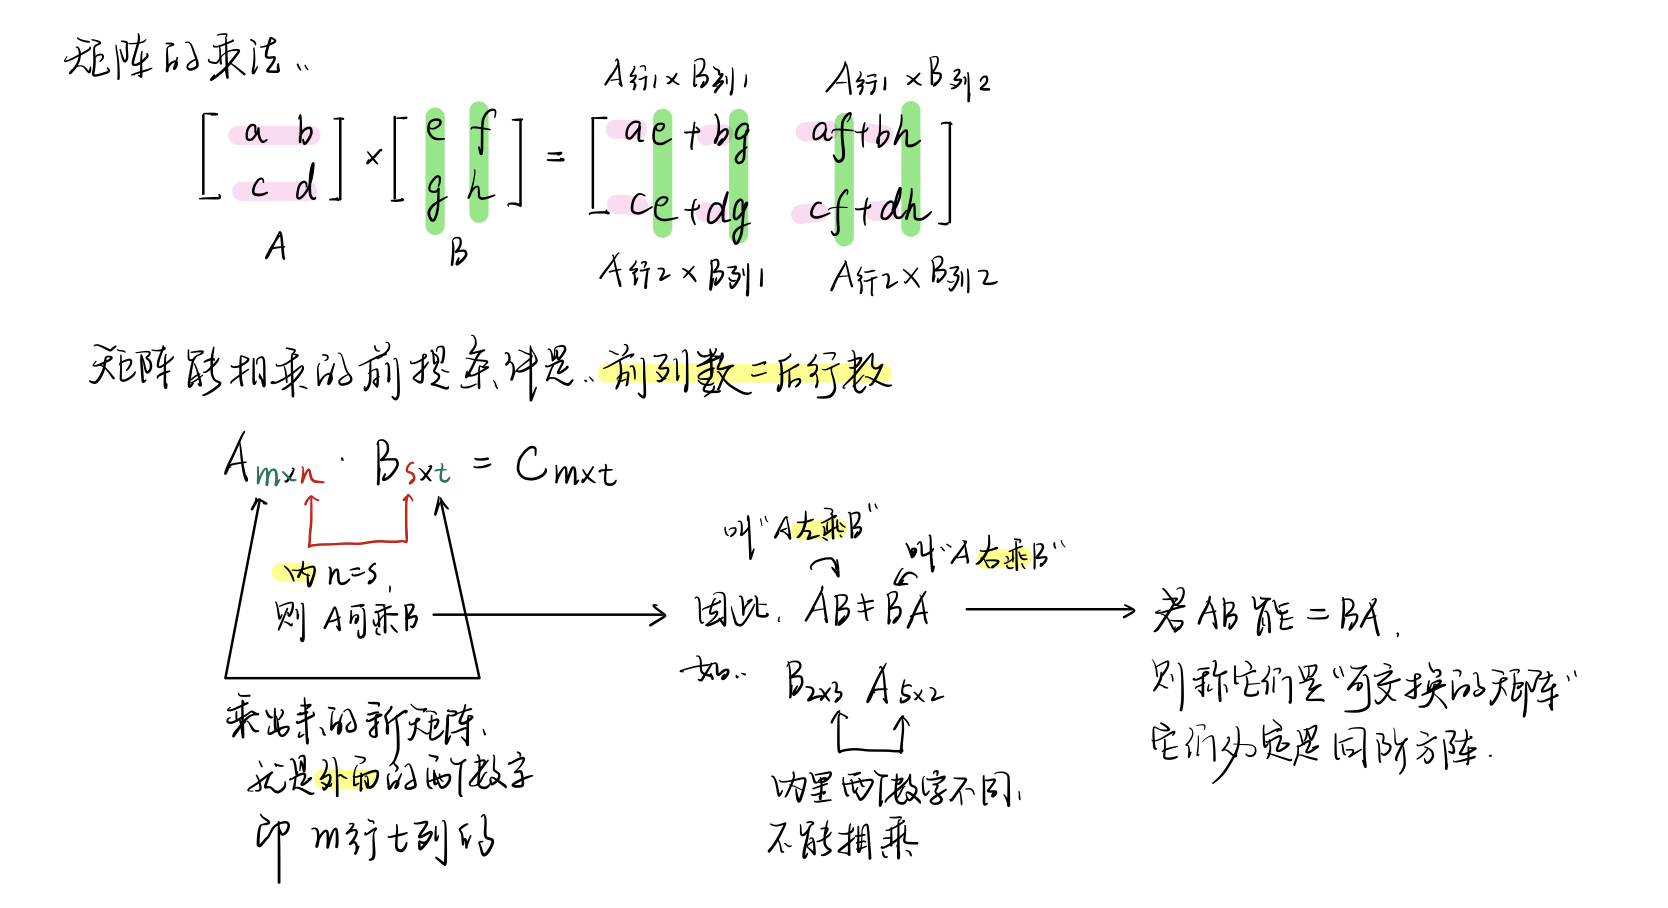
\includegraphics[width=1\textwidth]{img/0016.png} 

所以: \\
- 两个矩阵相乘的顺序不同的话, 结果就不同. 即: $AB \neq BA $ \\
- AB这个顺序能相乘, 不一定BA这个顺序也能相乘. 比如, $A_{5×2}B_{2×3}$ 是可以相乘的(它们内侧两个数字相同, 都是2), 能得到一个 5行3列的矩阵. 而顺序倒过来 $B_{2×3}A_{5×2}$就不能相乘了, 因为它们的内侧两个数字(前为3, 后为5)不相同. \\

所以, 我们要区分一下相乘的顺序: \\
- AB : 叫``A左乘B", 或``B右乘A" \\


单位阵E, 就相当于1的作用. 所以 AE = EA = A. 但是注意, 这里前后的两个单位阵E, 不是同一个E!  比如: \\
$A_{2×3}E_{3×3}=E_{2×2}A_{2×3}$\\
前面的E, 只能是3阶方阵. 后面的E, 只能是2阶方阵. 所以这两个E不是同一个单位阵. \\







\begin{myEnvSample}
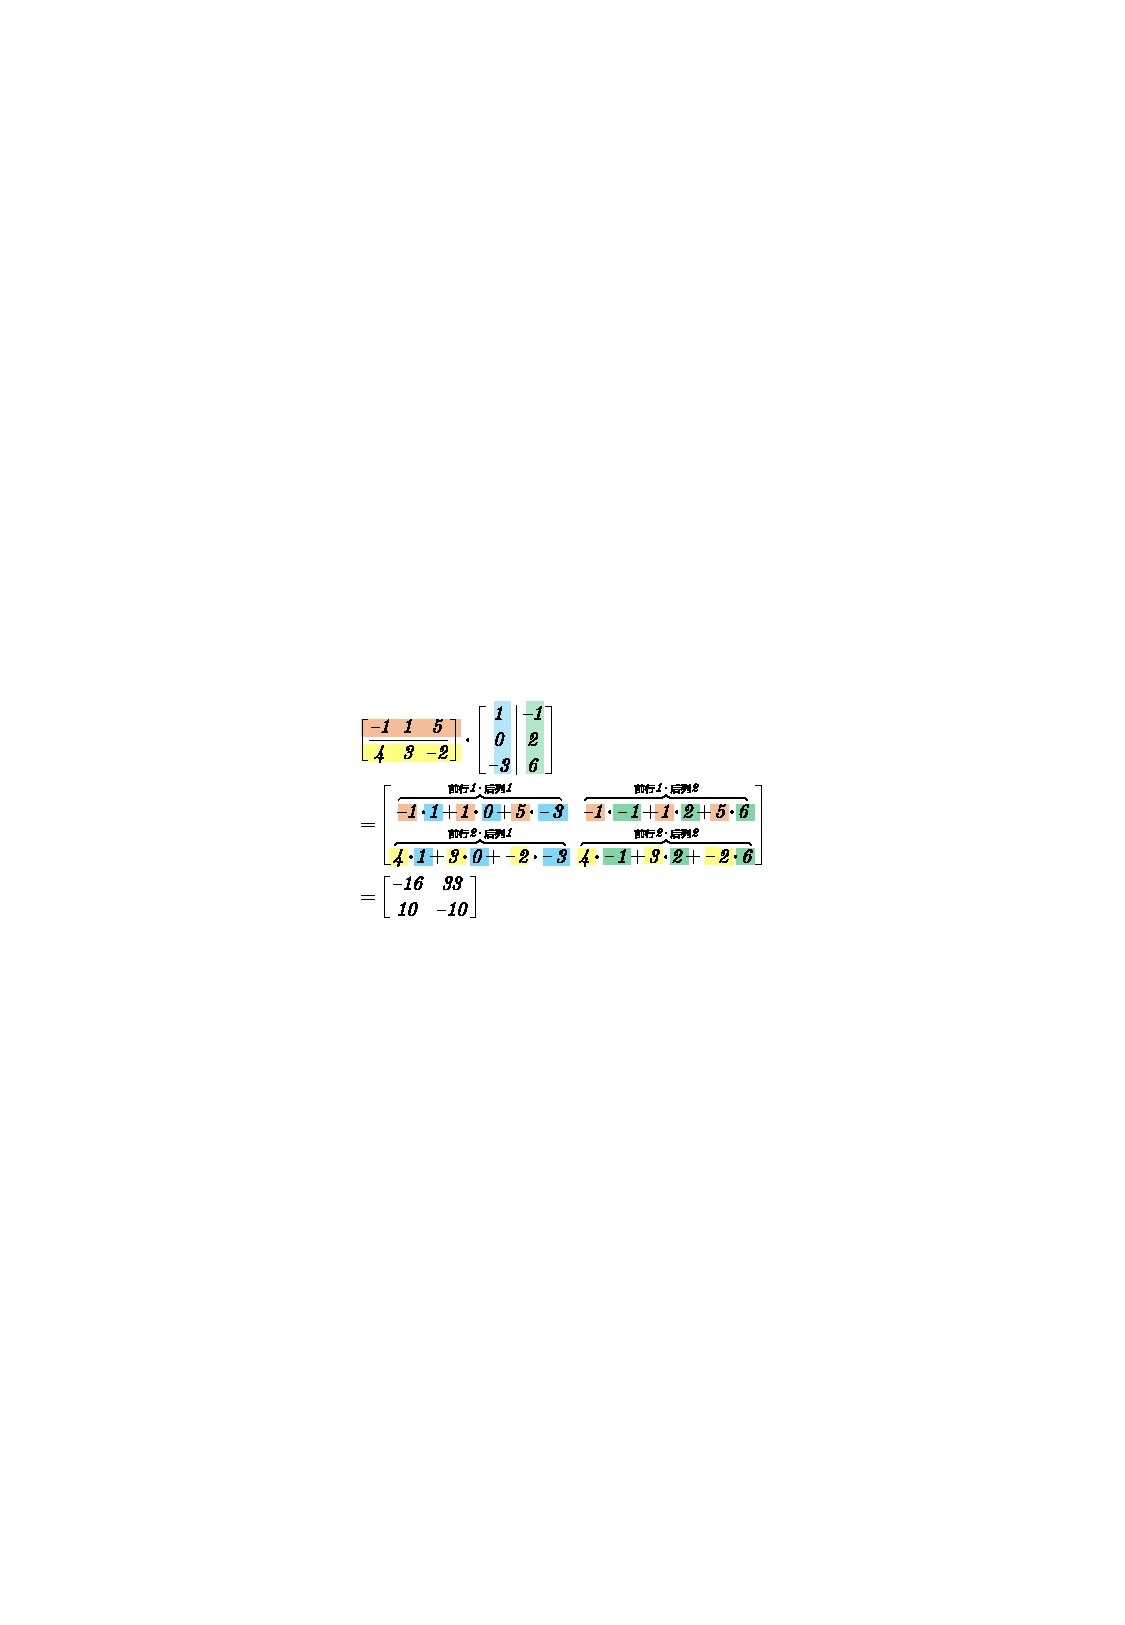
\includegraphics[width=0.6\textwidth]{img/0017.pdf}
\end{myEnvSample}

\hrule

\subsubsection{(1) AB=0 , 是推不出 A=0 或 B=0 的. (2) AB=AC, 且 $A =\neq 0 $, 是推不出 B=C 的.}

\begin{align*}
	& \text{有}	A=\left[ \begin{matrix}
		2&		0\\
		-1&		0\\
	\end{matrix} \right] ,\ B=\left[ \begin{matrix}
		0&		0\\
		1&		3\\
	\end{matrix} \right] ,\ C=\left[ \begin{matrix}
		0&		0\\
		2&		4\\
	\end{matrix} \right]\\
	&  \text{则:} AB=\left[ \begin{matrix}
		0&		0\\
		0&		0\\
	\end{matrix} \right] ,\ AC=\left[ \begin{matrix}
		0&		0\\
		0&		0\\
	\end{matrix} \right]\\
\end{align*}

从上面的结果, 我们可以得出这两个结论: \\
- \textbf{AB=0 , 是推不出 A=0 或 B=0 的.} \\
- \textbf{AB=AC, 且 $A \neq 0 $, 是推不出 B=C 的.} \\

\hrule

\subsubsection{一个矩阵, 与``零矩阵"相乘, 结果就是一个``新形状"的零矩阵}

如: $A_{4×3}O_{3×2}=O_{4×2}$ \\

\hrule

\subsubsection{一个矩阵X, 与``单位阵E"相乘(无论左乘还是右乘), 结果还是矩阵X本身. 即: AE=A, EB=B}

AE=A, EB=B \\

如: $
\underset{A}{\underbrace{\left[ \begin{matrix}
			3&		3&		3\\
			4&		1&		1\\
			5&		9&		9\\
		\end{matrix} \right] }}×\underset{E}{\underbrace{\left[ \begin{matrix}
			1&		&		\\
			&		1&		\\
			&		&		1\\
		\end{matrix} \right] }}=\underset{A}{\underbrace{\left[ \begin{matrix}
			3&		3&		3\\
			4&		1&		1\\
			5&		9&		9\\
		\end{matrix} \right] }}
$\\

\hrule

\subsection{矩阵乘法的运算规律}

\subsubsection{结合律: (AB)C = A(BC)} 

ABC的顺序, 在等号两边, 不变.\\


\subsubsection{分配律: (1) (A+B)C = AC+BC,  (2) C(A+B) = CA+CB} 

C在右边时, 分配进去, C还是在右边. \\
C在左边时, 分配进去, C还是在左边. \\


\subsubsection{ k(AB) = (kA)B = A(kB)} 

即 k乘以AB, 可以先和A结合来算, 也可以先和B结合来算. \\
并且无论k在哪, AB的左右顺序, 永远是AB. \\


\hrule

\subsubsection{矩阵乘法的例题}

\begin{myEnvSample}
求出 与$
A=\left[ \begin{matrix}
	1&		0\\
	1&		1\\
\end{matrix} \right] 
$ 可交换的所有矩阵.\\

设其可交换的矩阵 $
B=\left[ \begin{matrix}
	a&		b\\
	c&		d\\
\end{matrix} \right] \ 
$

B要能与A可交换, 它就必须满足: $A_n B_n = B_n A_n $, 即A和B是同阶的方阵.  \\

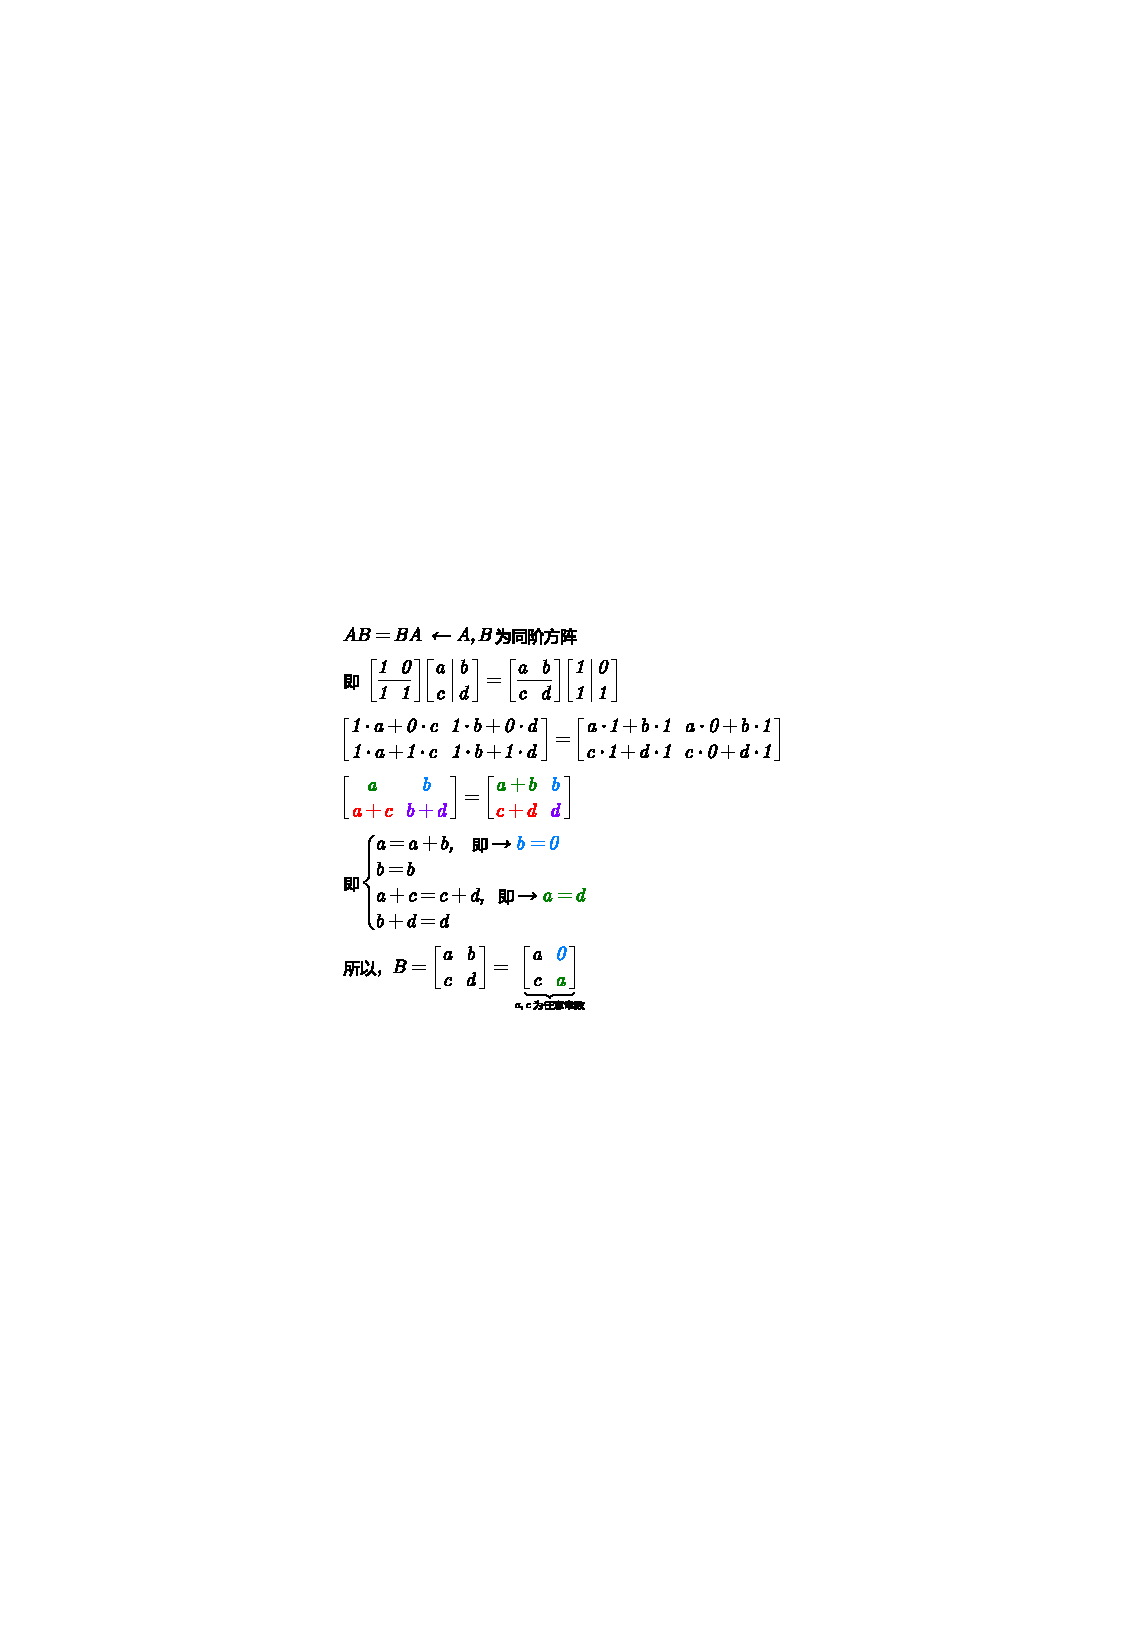
\includegraphics[width=0.7\textwidth]{img/0018.pdf}
\end{myEnvSample}




\begin{myEnvSample}
$
\left\{ \begin{array}{l}
	x_1=y_1-y_2\\
	x_2=y_1+y_2\\
\end{array} \right. \ \ \text{可以写成:\ }\left[ \begin{array}{c}
	x_1\\
	x_2\\
\end{array} \right] =\underset{\text{这两块,就是两个矩阵相乘}}{\underbrace{\left[ \begin{matrix}
			1&		-1\\
			\hline
			1&		1\\
		\end{matrix} \right] \left[ \begin{array}{c}
			y_1\\
			y_2\\
		\end{array} \right] }}
$
\end{myEnvSample}


\hrule

\subsection{矩阵, 幂的运算}
\subsubsection{$A^k=A\cdot A\cdot ...A\ ←\text{等号右边共}k\text{个}A$}

\begin{align*}
	A^k=\underset{k\text{个}A}{\underbrace{A\cdot A\cdot ...A}}
\end{align*}

\subsubsection{$A^0 = E$}

\subsubsection{$A^{k_1}A^{k_1}=A^{k_1+k_2}$}

\subsubsection{$\left( A^{k_1} \right) ^{k_2}=A^{k_1k_2}$}

\subsubsection{一般, $\left( AB \right) ^k\ne A^k B^k$ }

比如,  $\left( AB \right) ^2\ne A^2 B^2$ \\
因为: 等号左边 $\left( AB \right) ^2=\ ABAB$, 等号右边 $A^2B^2=\ AABB$, 而一般 $ABAB \ne AABB$. 因为虽然它们最左边都是A, 最右边都是B, 但是中间的两个矩阵相乘, BA一般就不等于AB了. 除非它们是可交换矩阵. \\

其他的: \\
$\left( A+B \right) ^2\ne A^2+2AB+B^2$  ← 这个, 一般也不相等 \\
$\left( A-B \right) ^2\ne A^2-2AB+B^2$  ← 这个, 一般也不相等 \\

\begin{myEnvSample}
问 $\left( A+E \right) ^2$ 是否等于 $A^2+2AE+E^2$ ?

\begin{align*}
		& \left( A+E \right) ^2=\left( A+E \right) \left( A+E \right)\\
	& =A\left( A+E \right) +E\left( A+E \right)\\
	& =A^2+\underset{=A}{\underbrace{AE}}+\underset{=A}{\underbrace{EA}}+\underset{=E}{\underbrace{E^2}}\\
	& =A^2+\underset{=2AE}{\underbrace{2A}}+E
\end{align*}

所以这个是对的. 相等. 
\end{myEnvSample}

同样, $\left( A-E \right) ^2 = A^2-2AE+E^2$ \\

\hrule

\subsubsection{矩阵的幂运算 例题}

\begin{myEnvSample}
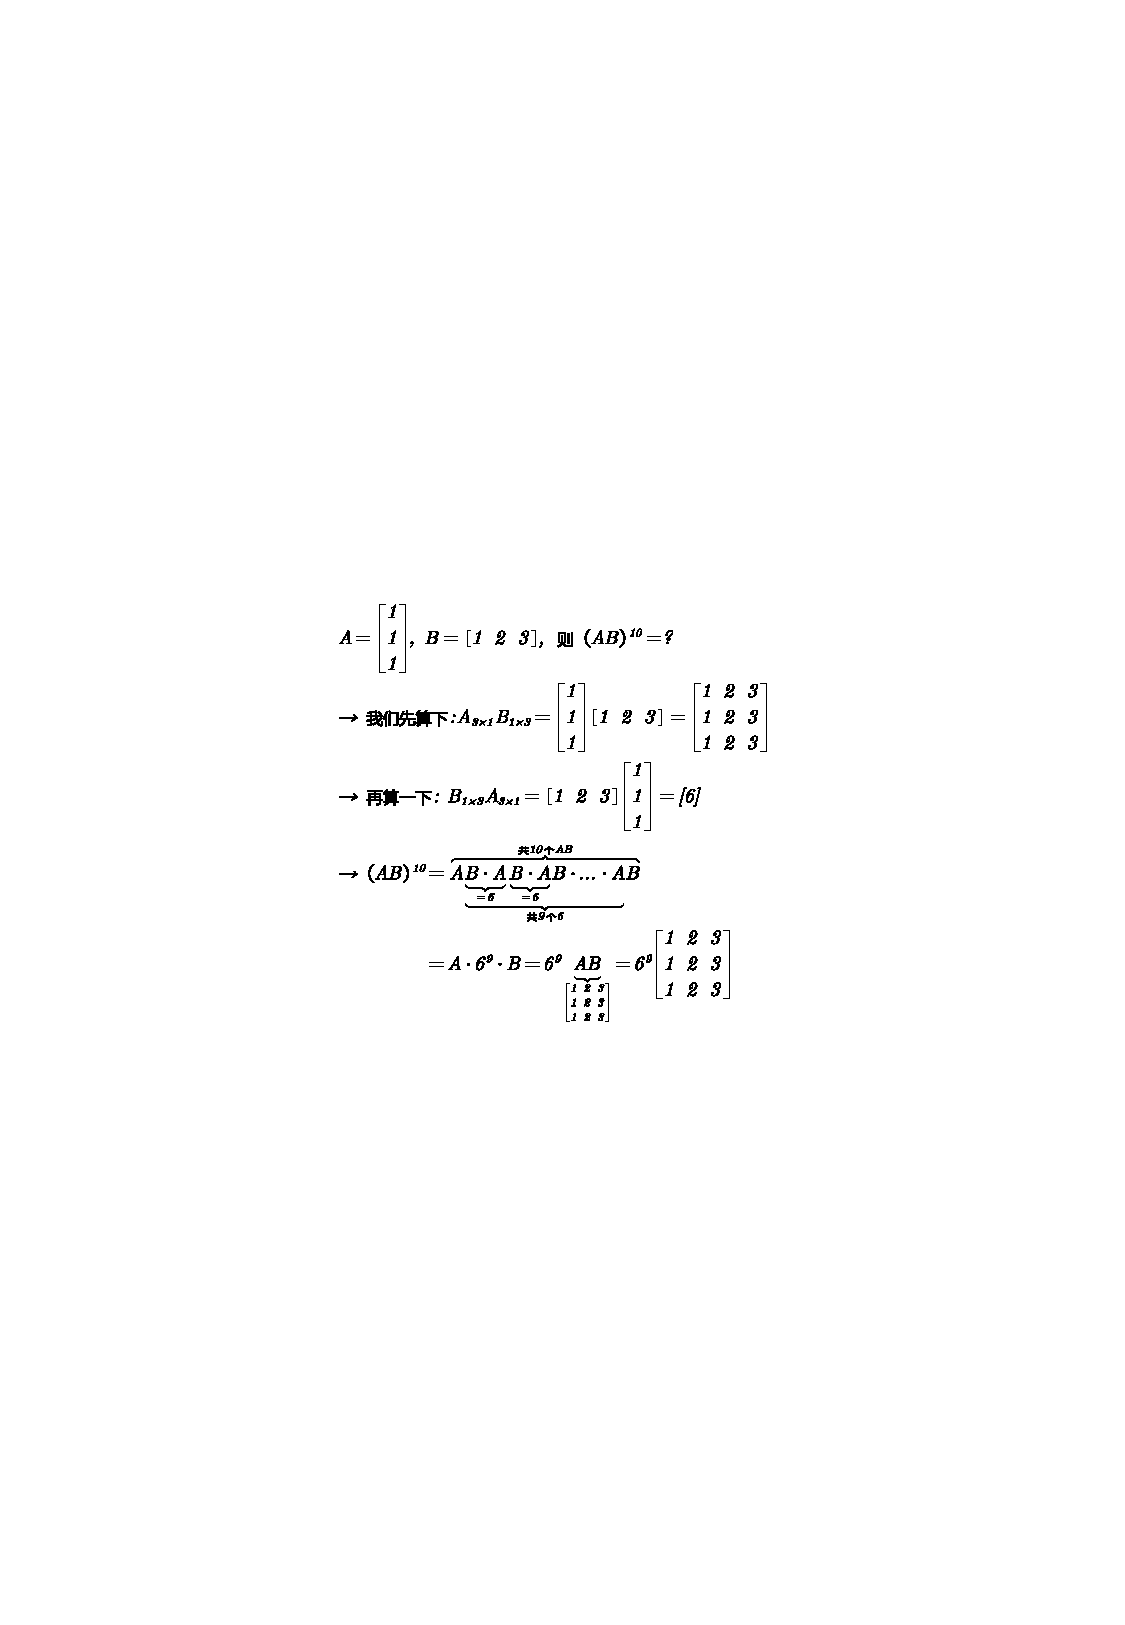
\includegraphics[width=0.6\textwidth]{img/0019.pdf}
\end{myEnvSample}


\hrule

\section{矩阵的转置}

$A_{m×n}$, 转置后, 就是$(A^T)_{n×m}$ \\

\subsection{性质: $(A^T) ^T = A$ }

\subsection{性质: $(A+B) ^T = A^T + B^T$ }

\subsection{性质: $(kA) ^T =  kA^T$ }

\subsection{\ding{72} 性质: $(AB) ^T = B^T A^T$  ← 注意AB顺序要颠倒 }

\subsection{性质: $(A_1 A_2 A_3 A_4)^T = A_4^T  A_3^T  A_2^T  A_1^T$ ← 顺序颠倒}

\hrule


\section{特殊矩阵 (都是方阵)}

\subsection{数量矩阵}

数量矩阵(或叫``纯量阵") scalar matrix : 就是``主对角线上"元素都是同一个数值,其余元素都是零. \\
即: \\
$
\left[ \begin{matrix}
	a&		&		&		\\
	&		a&		&		\\
	&		&		\ddots&		\\
	&		&		&		a\\
\end{matrix} \right]  
= aE
$\\

所以, 零矩阵, 和单位阵E, 都是特殊的``数量矩阵". \\

有性质: \\
(aE)B = B(aE) = aB \\


\hrule


\subsection{对角型矩阵}

对角矩阵 diagonal matrix : 主对角线元素无要求(可以不相等), 但之外的所有元素都为0.\\

即: 
\begin{align}
	A\ =\left[ \begin{matrix}
		\lambda _1&		&		&		\\
		&		\lambda _2&		&		\\
		&		&		\ddots&		\\
		&		&		&		\lambda _n\\
	\end{matrix} \right]
\end{align}

可记为: $A = diag(\lambda_1, \lambda2, ..., \lambda_n) $\\

所以, ``数量矩阵"(主对角线上的元素都相等), 只不过是一种特殊的``对角矩阵"罢了.\\




\subsubsection{diag × B : 对角阵元素在哪一行上, 就乘到B的相同行上去}

\begin{align}
	\left[ \begin{matrix}
		k_1&		&		\\
		\hline
		&		k_2&		\\
		\hline
		&		&		k_3\\
	\end{matrix} \right] \left[ \begin{matrix}
		1&		2&		3\\
		\hline
		2&		2&		2\\
		\hline
		8&		8&		8\\
	\end{matrix} \right] =\left[ \begin{matrix}
		1k_1&		2k_1&		3k_1\\
		\hline
		2k_2&		2k_2&		2k_2\\
		\hline
		8k_3&		8k_3&		8k_3\\
	\end{matrix} \right]
\end{align}

即: diag 在前, 就乘到后者的``行"上去. (前行,后列) \\
即: \textbf{左乘, 对应后面的行.}\\




\subsubsection{B × diag : 对角阵元素在哪一列上, 就乘到B的相同列上去}

\begin{align}
	\left[ \begin{array}{c|c|c}
		1&		2&		3\\
		2&		2&		2\\
		8&		8&		8\\
	\end{array} \right] \left[ \begin{array}{c|c|c}
		k_1&		&		\\
		&		k_2&		\\
		&		&		k_3\\
	\end{array} \right] =\left[ \begin{array}{c|c|c}
		1k_1&		2k_2&		3k_3\\
		2k_1&		2k_2&		2k_3\\
		8k_1&		8k_2&		8k_3\\
	\end{array} \right]
\end{align}

即: diag 在后, 就乘到前者的``列"上去. (前行,后列)\\
即: \textbf{右乘, 对应后面的列.} \\

\hrule


\subsection{上三角形矩阵}

upper triangular matrix \\

$
\left[ \begin{matrix}
	a_{11}&		a_{12}&		a_{13}&		a_{14}\\
	&		a_{22}&		a_{23}&		a_{24}\\
	&		&		\ddots&		a_{34}\\
	&		&		&		a_{44}\\
\end{matrix} \right] 
$ \\

性质: \\
- 上三角矩阵, 乘以系数后, 也是上三角矩阵 \\
- 上三角矩阵间的``加减法"和``乘法"运算的结果, 仍是上三角矩阵 \\
- 上三角矩阵的``逆矩阵", 也仍然是上三角矩阵 \\
- 上三角矩阵的行列式, 为``主对角线"元素相乘 


\subsection{下三角形矩阵}

$
\left[ \begin{matrix}
	a_{11}&		&		&		\\
	a_{21}&		a_{22}&		&		\\
	a_{31}&		a_{32}&		\ddots&		\\
	a_{41}&		a_{42}&		a_{43}&		a_{44}\\
\end{matrix} \right] 
$\\


\hrule


\subsection{对称矩阵: 有 $A^T = A$ ← 即对自己做转置, 依然等于自己.}

对称矩阵 Symmetric Matrices : 是以主对角线为对称轴, 上下元素对应相等. 即: $a_{ij}= a_{ji}$ \\

如:\\
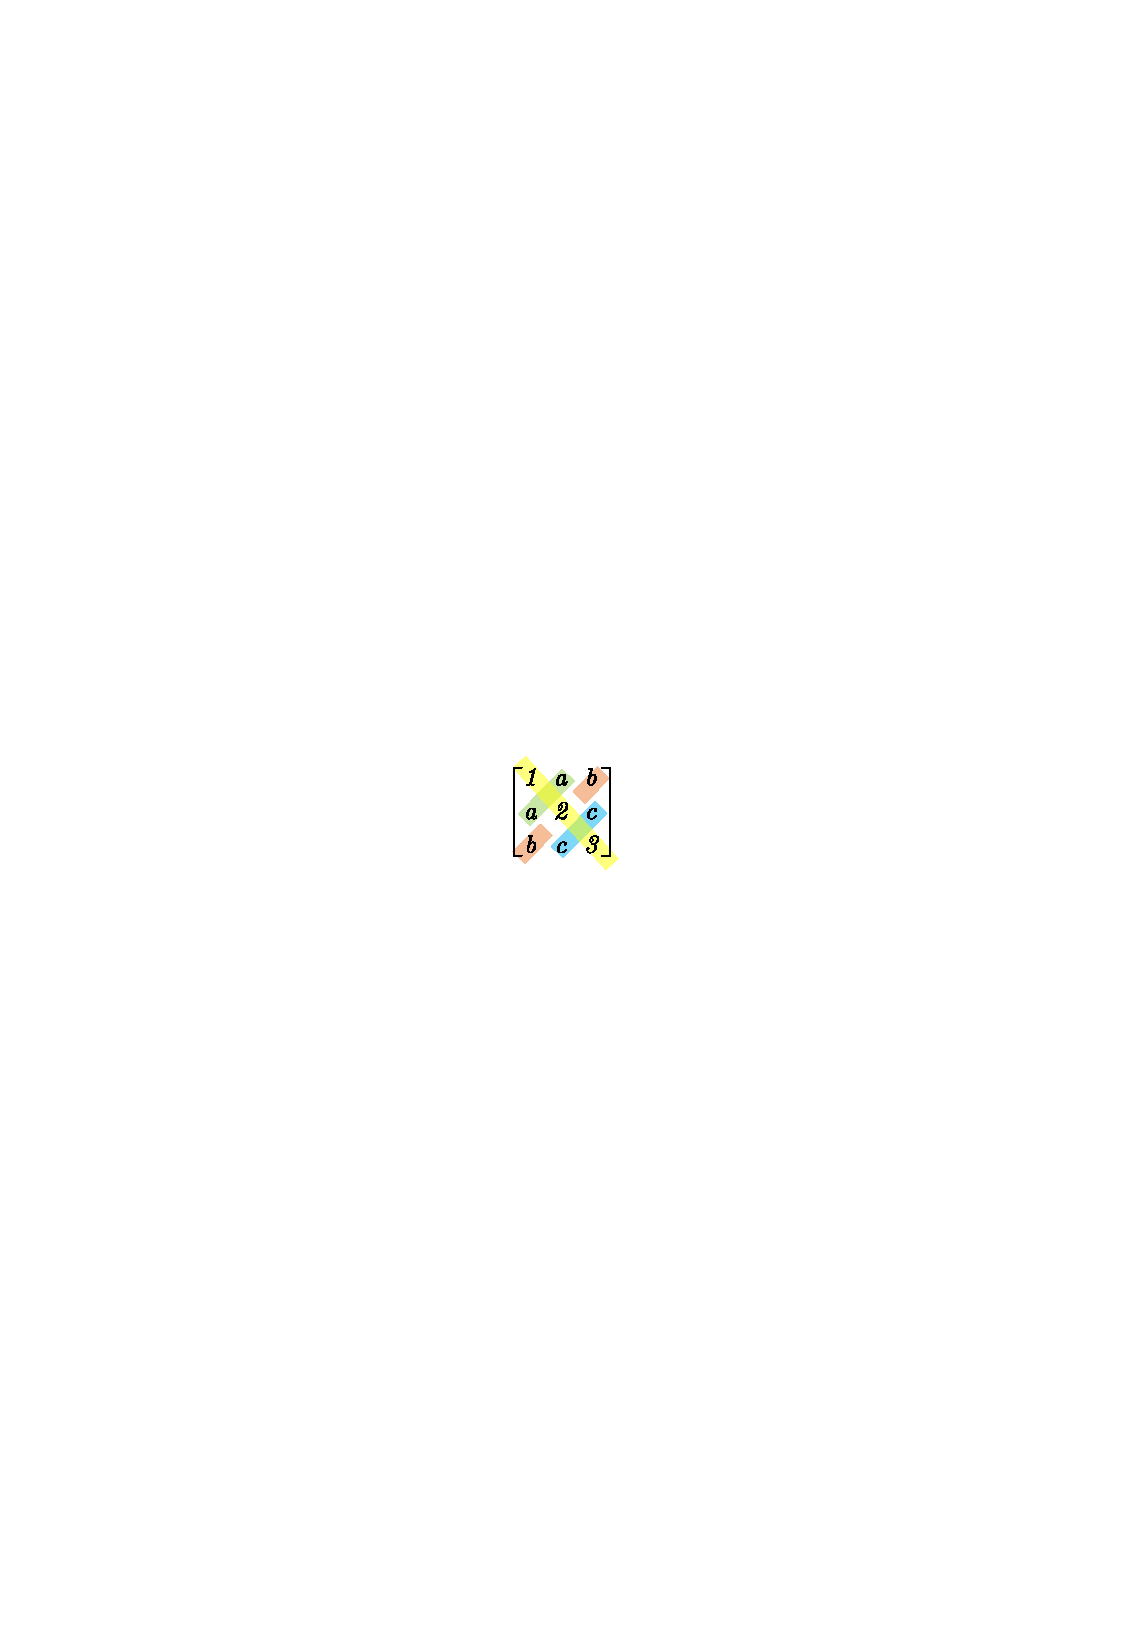
\includegraphics[width=0.15\textwidth]{img/0020.pdf}\\

对称矩阵, 有性质: $A^T = A$ \\



\begin{myEnvSample}
	注意: 下面例题中的字打错了, 不是``互为", 而是``都是". \\
	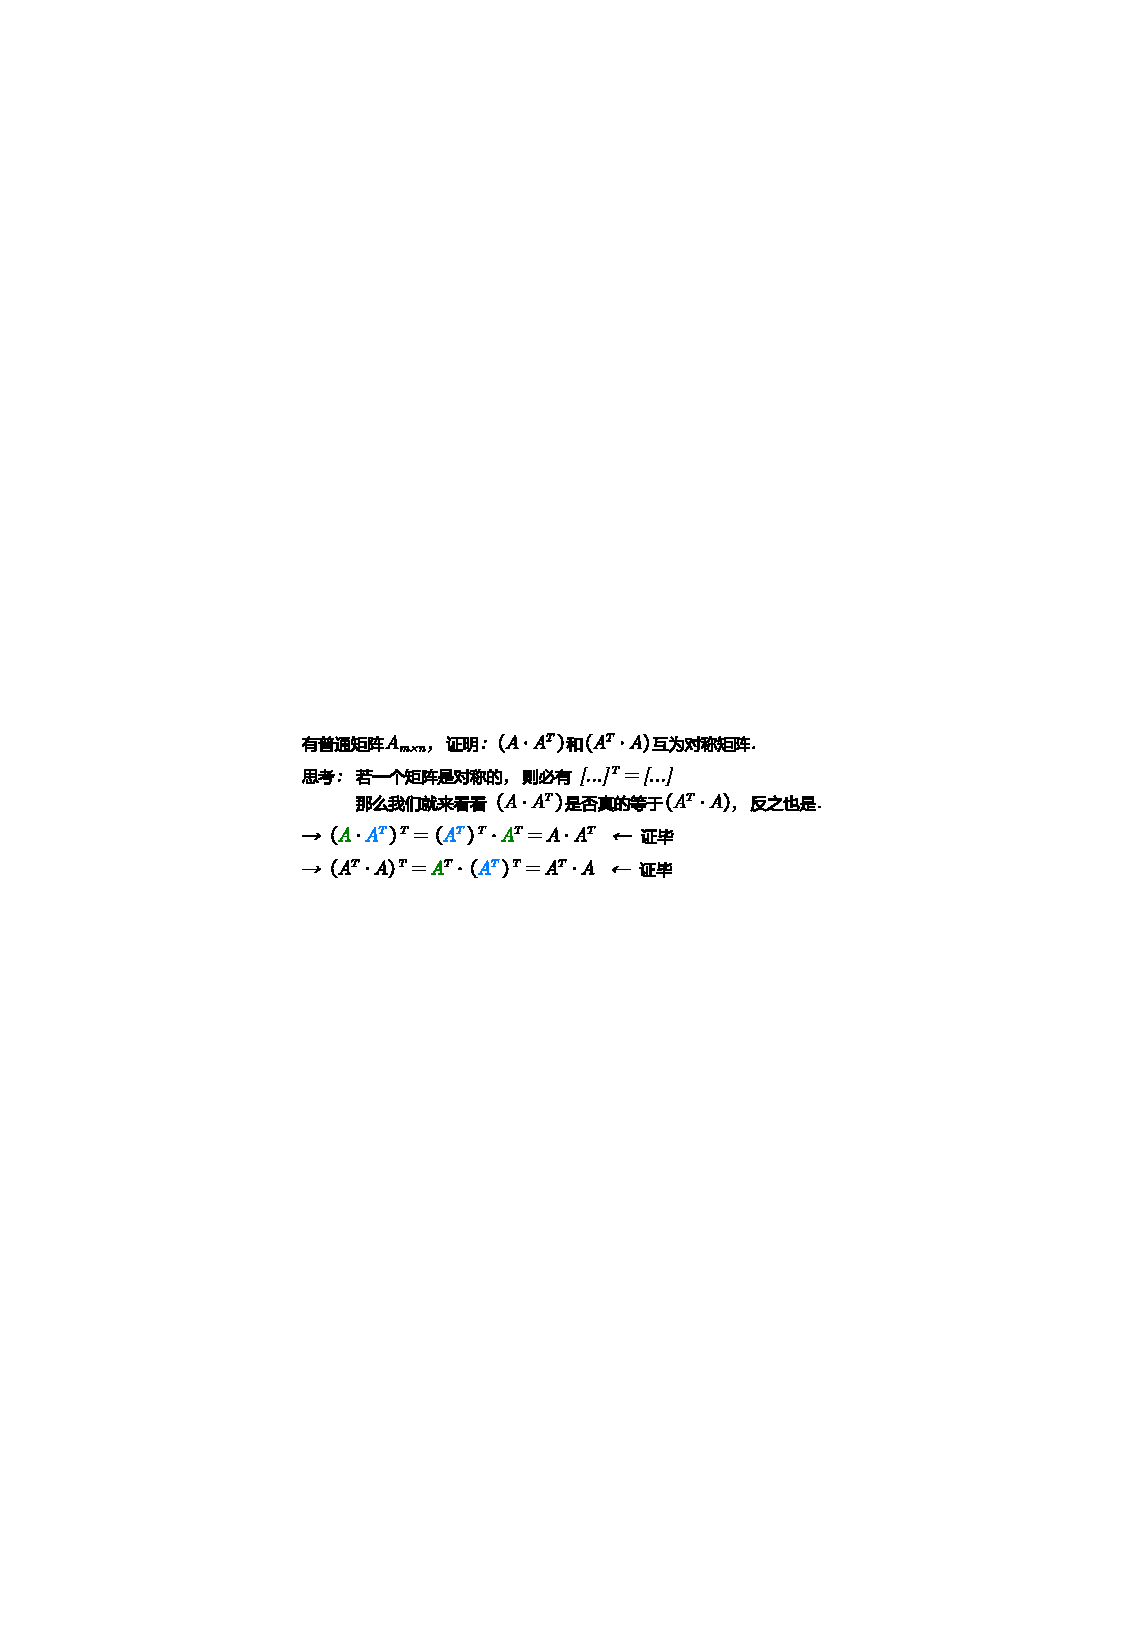
\includegraphics[width=0.75\textwidth]{img/0021.pdf}
\end{myEnvSample}



\begin{myEnvSample}
	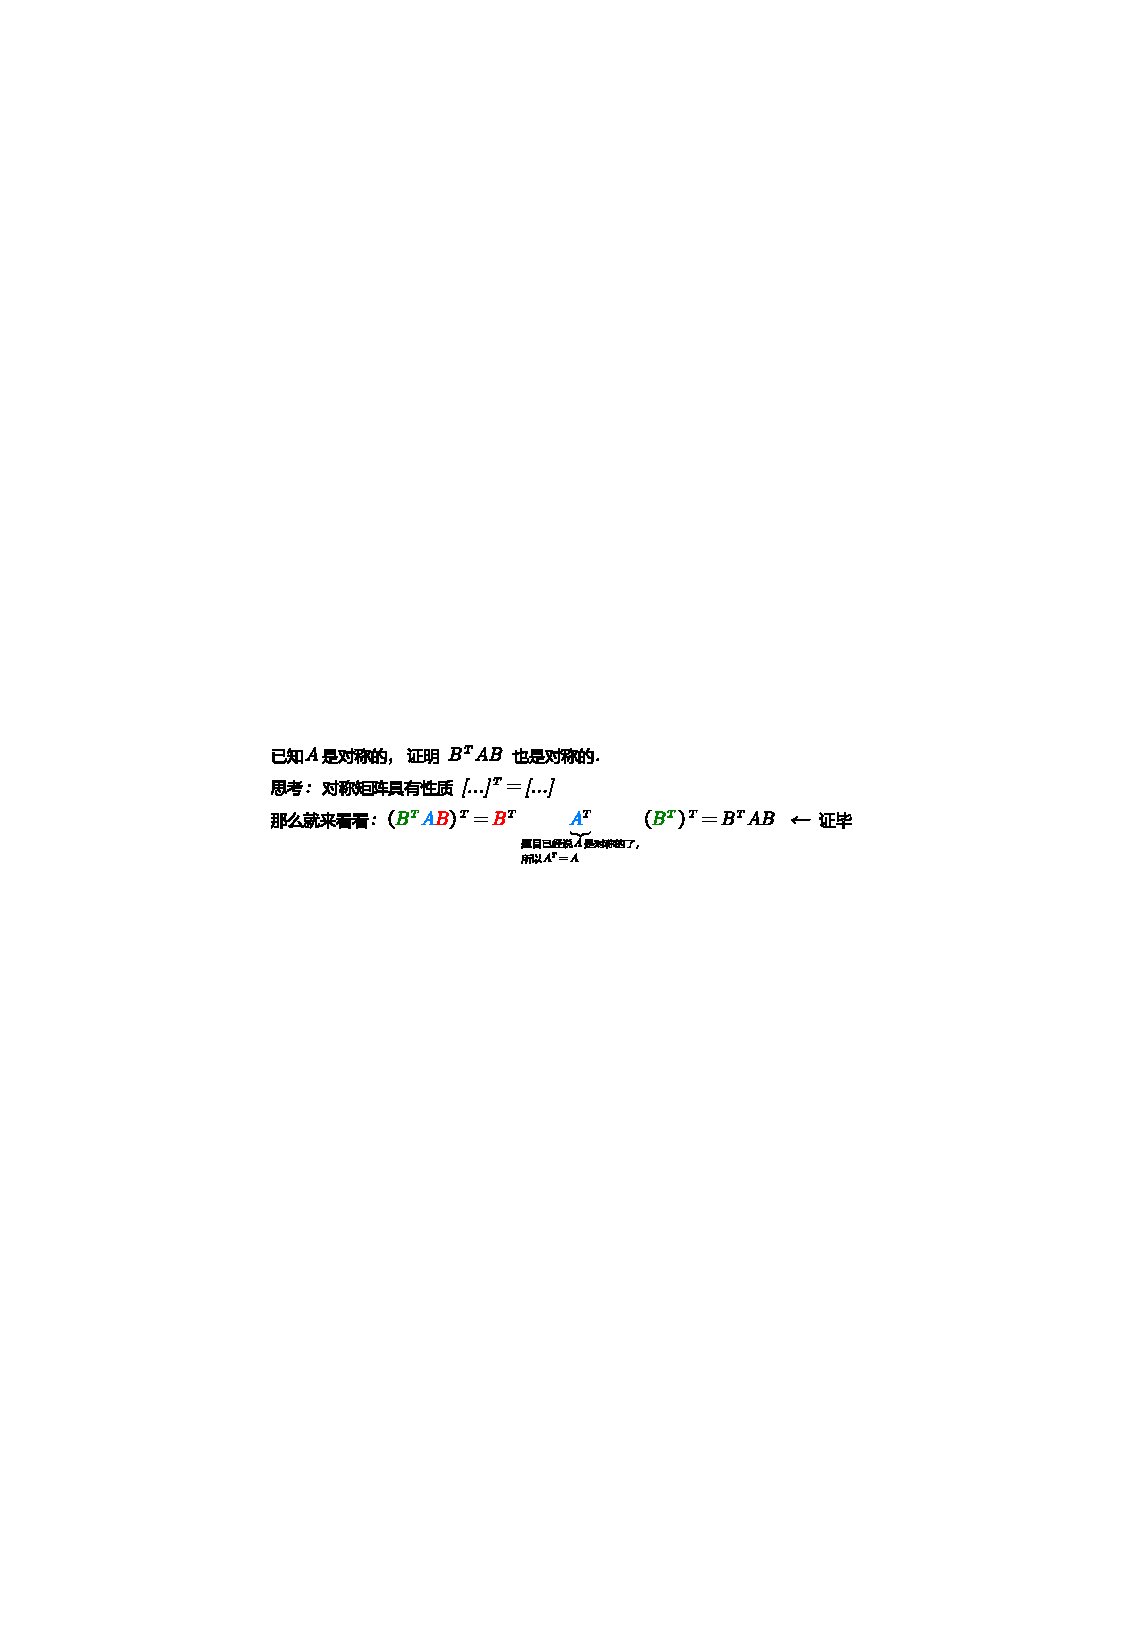
\includegraphics[width=0.8\textwidth]{img/0022.pdf}
\end{myEnvSample}





A,B 是同阶的``对称矩阵", 则有性质: 

\subsubsection{性质: $\left( A+B \right) ^T=A^T+B^T=A+B$ }

$
\left( A+B \right) ^T=\underset{A^T=A}{\underbrace{A^T}}+\underset{B^T=B}{\underbrace{B^T}}=A+B
$


\subsubsection{性质: $\left( A-B \right) ^T=A^T-B^T=A-B$ }


\subsubsection{性质: $\left( kA \right) ^T=k\cdot A^T=kA$ }

$
\left( kA \right) ^T=k\cdot \underset{A^T=A}{\underbrace{A^T}}=kA
$


\subsubsection{性质: $\left( AB \right) ^T=B^TA^T=BA\ne AB$ }

$
\left( AB \right) ^T=\underset{B^T=B.}{\underbrace{B^T}}\underset{A^T=A}{\underbrace{A^T}}=BA\ne AB
$


\subsubsection{定理: 两个对称矩阵A,B 相乘后, 新矩阵AB 一般就不再是对称的了. 除非A,B 是可交换矩阵, 型矩阵AB 才是对称的.}

即: 对称矩阵A, B, 只有在它们是``可交换矩阵"的前提下, 它们的乘积A×B, 才也是``对称矩阵". \\


\hrule


\subsection{反对称矩阵 : 有 $A^T = - A$}

反对称矩阵 Skew-symmetric matrix : 主对角线上的元素全为零,主对角线两侧对称的元素, 反号(即互为相反数). 即 $a_{ij}= -a_{ij}$ \\

如: \\
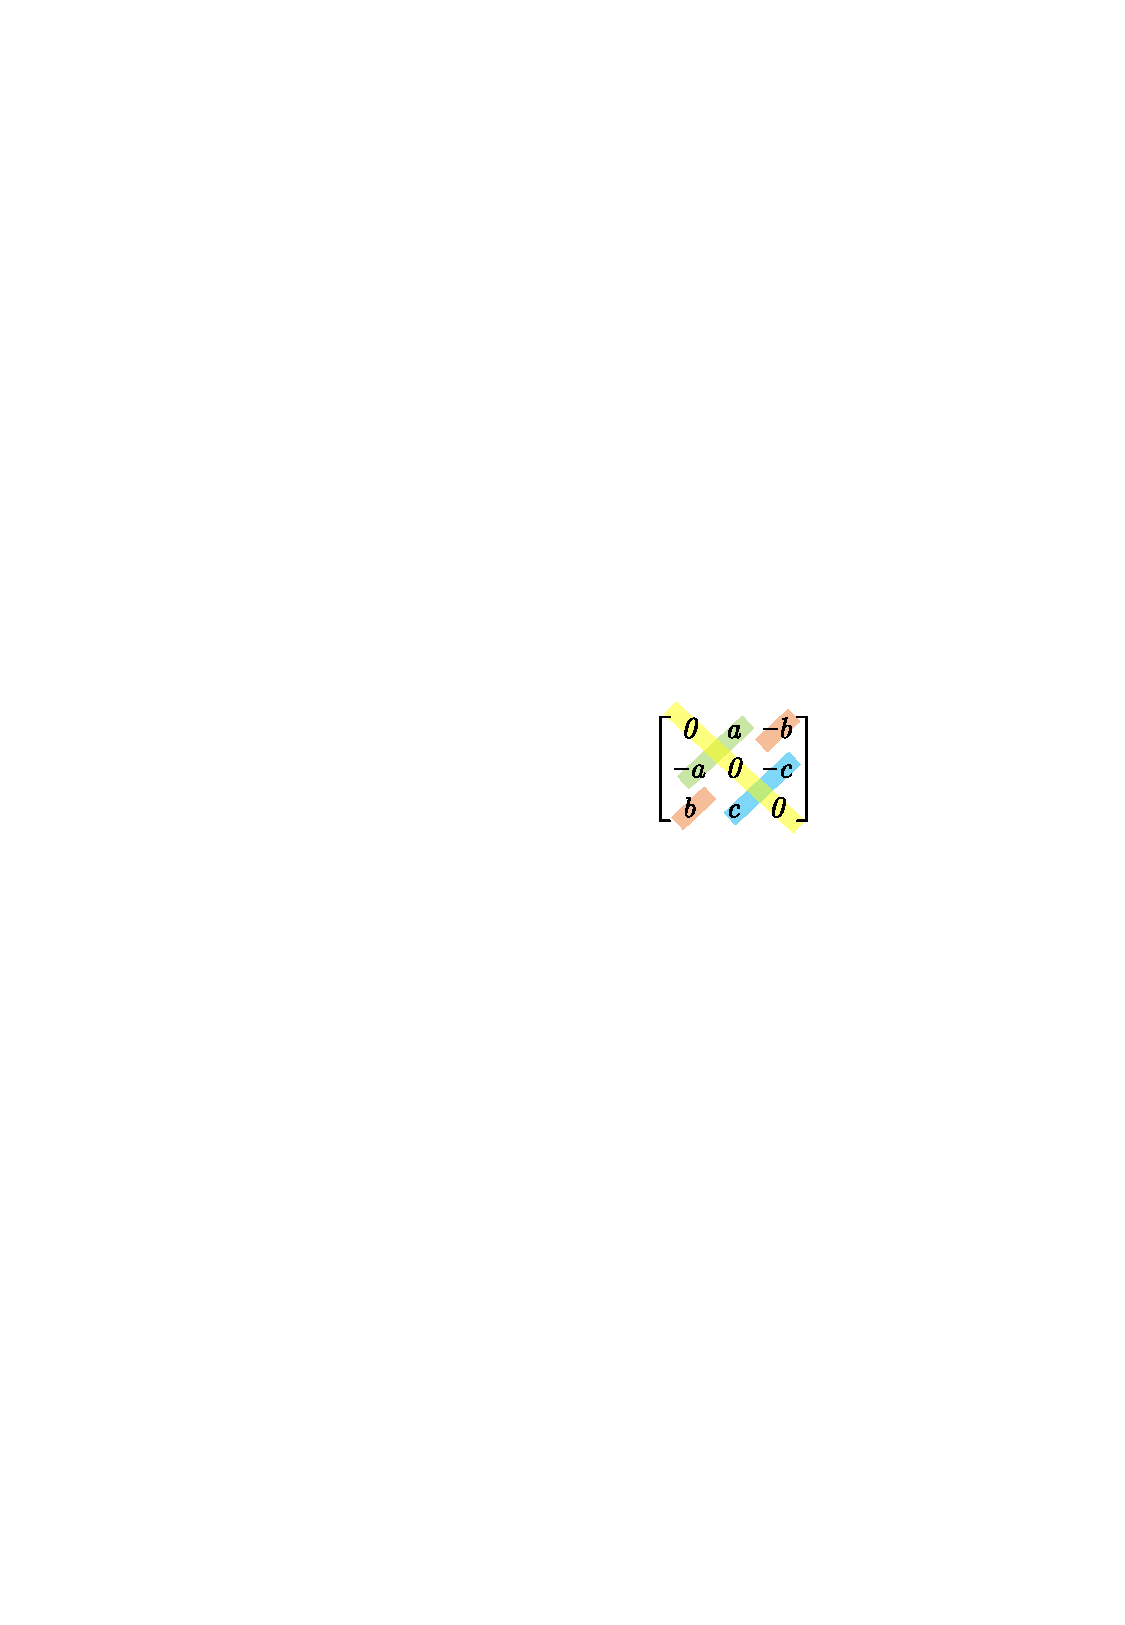
\includegraphics[width=0.15\textwidth]{img/0023.pdf} \\

为什么它主对角线上的元素都是0呢? 因为根据``反对称矩阵"的性质: $a_{ii}= -a_{ii}$, 则就 $2a_{ii}=0$, 所以就有 $a_{ii}=0$ 了. \\

反对称矩阵, 有性质: $A^T = - A$.\\


\hrule


\section{逆矩阵}

要记住一句话: 线性代数中,\textbf{矩阵不能放在分母上!} \\


\hrule



\section{方阵的行列式}

只需把矩阵的中括号, 改成行列式的两条竖线, 就得到了``方阵的行列式". \\
如: 矩阵$
A=\left[ \begin{matrix}
	1&		1&		1\\
	2&		2&		2\\
	3&		3&		3\\
\end{matrix} \right] 
$, 其行列式就是: 
$
|A|=\left| \begin{matrix}
	1&		1&		1\\
	2&		2&		2\\
	3&		3&		3\\
\end{matrix} \right|
$\\

行列式和矩阵有什么关系? 其实, 行列式只是矩阵的一个``属性"而已. \\
矩阵有很多属性, 包括: 特征值, 特征向量, 行列式, 等等. \\



\subsection{``方阵的行列式"的性质}

\subsubsection{性质: $|A^T|=|A|$}

\subsubsection{  \ding{72} 性质: $|kA|=k^n|A|$}

\subsubsection{性质: $|AB|=|A| \cdot |B|$ ← A,B 是同阶方阵}

因此,$|ABC|=|A|\cdot |B|\cdot |C|$\\

\begin{myEnvSample}
A是5阶方阵, 且|A|=3. 求:  \\
$
\ |-A|=|-1\cdot A|=-1^5\underset{=3}{\underbrace{|A|}}=-3
$\\
$
|2A^T|=2^5\underset{=|A|=3}{\underbrace{|A^T|}}=2^5\cdot 3=96
$\\
$
\left| \underset{=3}{\underbrace{\left| A \right|}}A \right|=3^5\underset{=3}{\underbrace{|A|}}=3^6
$\\

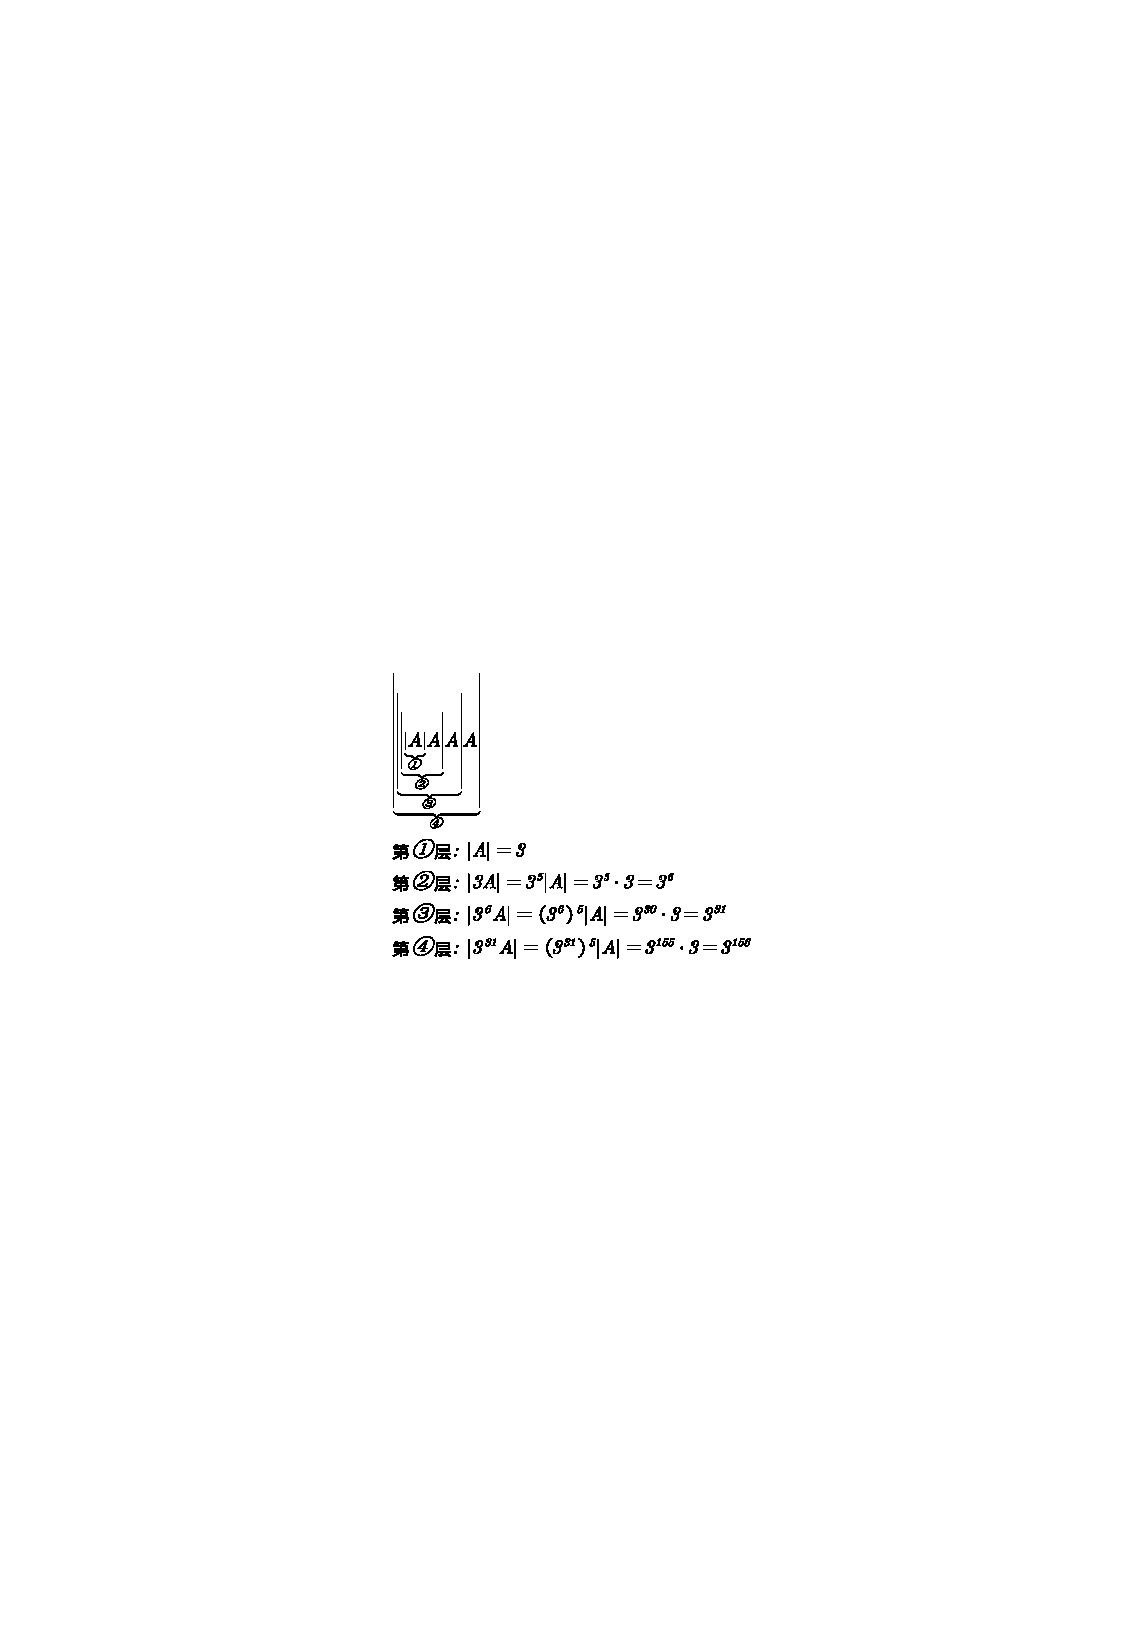
\includegraphics[width=0.55\textwidth]{img/0024.pdf}
\end{myEnvSample}



\hrule


\section{伴随矩阵  $A^*$}

\textbf{只有方阵, 才有伴随矩阵} Adjugate matrix. 并且任何方阵, 都有伴随矩阵.

如: $A=\left[ \begin{matrix}
	1&		1&		1\\
	\hline
	2&		1&		3\\
	\hline
	1&		1&		4\\
\end{matrix} \right] $ , 它的伴随矩阵 $A^*$ 是什么? \\

第1步: 先求出每个元素的``代数余子式": \\
$
A_{ij}=\left[ \begin{matrix}
	A_{11}=1&		A_{12}=-5&		A_{13}=1\\
	A_{21}=-3&		A_{22}=3&		A_{23}=0\\
	A_{31}=2&		A_{32}=-1&		A_{33}=-1\\
\end{matrix} \right]
$\\

第2步: 把$ A_{ij}$ 做转置, 就能得到A的伴随矩阵 $A^*$ :\\
$
A^*=\left[ \begin{array}{c|c|c}
	1&		-3&		2\\
	-5&		3&		-1\\
	1&		0&		-1\\
\end{array} \right]
$\\

即: 按``行"求的``代数余子式", 按``列"放. \\
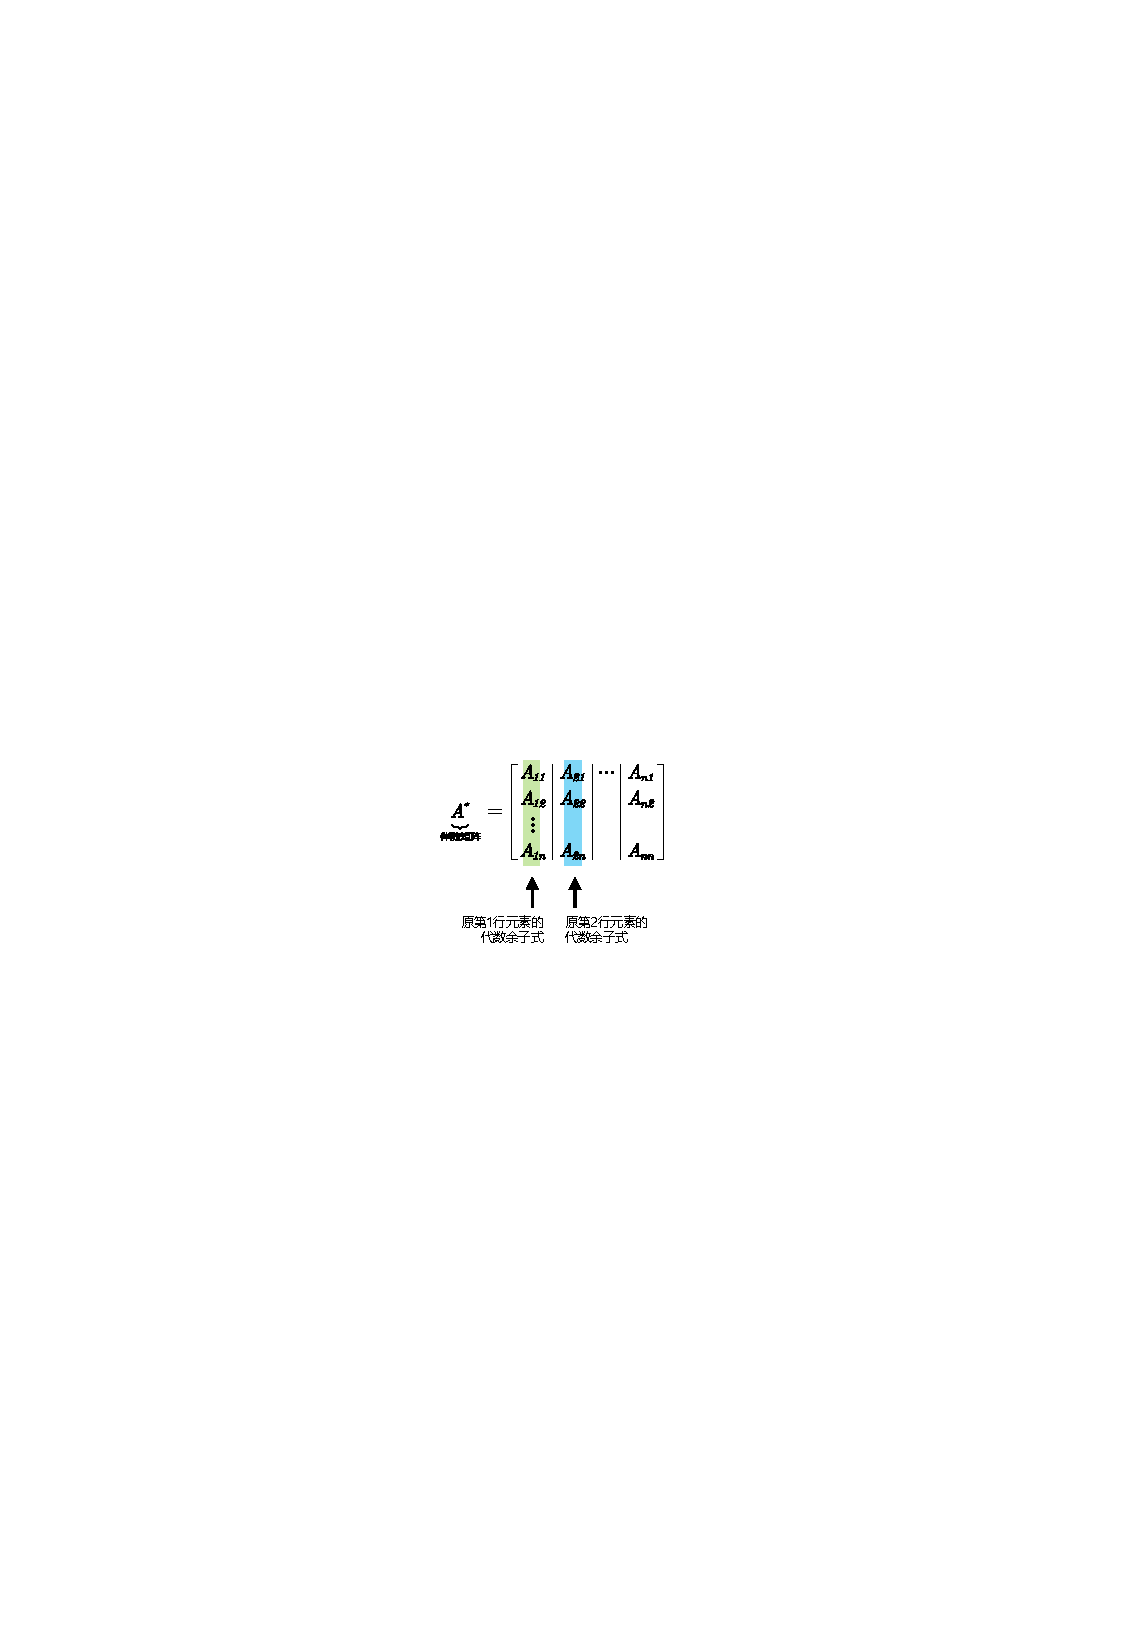
\includegraphics[width=0.35\textwidth]{img/0025.pdf}\\


\hrule


\subsection{伴随矩阵的性质}

\subsubsection{性质: 对``任意"方阵A, 有: $A * A^{\ast} = A^{\ast} * A = |A|E$}






https://www.bilibili.com/video/BV1aW411Q7x1?p=12&spm_id_from=pageDriver&vd_source=52c6cb2c1143f8e222795afbab2ab1b5

36.39



	
\end{document}